\documentclass{article}

\include{journal_definitions}
\usepackage[a4paper]{geometry}
\usepackage{hyperref}
\usepackage{graphicx}
\renewcommand{\figurename}{Figura}

\title{Como ver o invisible}
\author{Pablo Lemos}

\begin{document}
\maketitle

Seguro que algunha vez escoitastes falar da materia escura. Pode que incluso escoitaras, 
que so sabemos de que esta feito aproximadamente un cinco percento do Universo, e 
que miraras algún gráfico como o da figura \ref{fig:piechart}, que mostra a nosa 
ignorancia sobre o outro $95 \%$. É verdade, a maioría do Universo son cousas que non 
coñecemos nin entendemos. E se o pensas ben, ten moito sentido. Estamos observando dende 
un pequeno planeta, que da voltas o redor dunha pequena estrela, que da voltas dentro 
dunha Galaxia, que se move entre outros millóns de galaxias. ¡Non podemos queixarnos de 
que dende o noso planeta, só teñamos una pequena fracción dos compoñentes do cosmos!

\begin{figure}[h]
\includegraphics{piechart.pdf}
\caption{Esta figura representa os distintos compoñentes do Universo. En azul claro están 
os átomos, como os que forman todos os elementos que coñecemos. En verde está a materia 
escura, e en azul a enerxía escura. Non sabemos en que consisten ningún dos dous. 
Imaxe: \url{https://wmap.gsfc.nasa.gov/universe/uni_matter.html}
\label{fig:piechart}
}
\end{figure}


Pero se algunha vez escoitastes todo isto, e se tes unha mente curiosa, é posible que 
pensaras: ¿Como sabemos de que está feito o Universo? ¿De onde saen isos números? 
¿Acaso os científicos inventamos ese $4.6 \%$ para que nos sigan pagando? Evidentemente non. 
Esas preguntas e outras similares son as que intenta responder o campo da cosmoloxía. 
E se estás pensando que debe ser difícil responder esas preguntas, tes toda a razón. 
De feito, é tan difícil que a cosmoloxía non existía como disciplina científica ata ai un 
século, cando Einstein publicou a súa teoría da relatividade, que tiña como obxectivo describir 
as leis que describen todo o cosmos. 

Dende entón, pouco a pouco, comezamos a descifrar o enigma das estrelas. Démonos conta de 
que moitos dos puntos brillantes que vemos pola noite non son estrelas, senón galaxias con 
centos de millóns de estrelas cada una. Démonos conta de que pouco a pouco esas galaxias están 
afastándose da nosa, e que dentro de millóns de anos non poderemos velas. E démonos conta de 
que a maioría da materia do Universo non pódese ver (de aí o nome `materia escura'). E se estás pensando, mentres les isto, que é todo mentira, que soa a novela de ciencia ficción, 
neste artigo vou tratar de convencerte de que a materia escura e real. E vou tratar de convencerte 
da forma máis eficaz posible: Voute ensinar a materia escura. 

¿Como vou facer iso? ¿Como pretendo ensinarte o invisible? Se o pensas, é lóxico: Vou usar lentes. 
¿Que pasa cando ves una imaxe a través dunha lente? A lente distorsiona a imaxe, as veces faina 
parecer máis grande ou pequena, outras veces estira a imaxe nunha certa dirección. Se observamos 
una galaxia moi lonxe, toda a materia escura que está entre nos e a galaxia distorsiona a imaxe que 
vemos, igual que farían unas lentes de tamaño cósmico.

\begin{figure}[h]
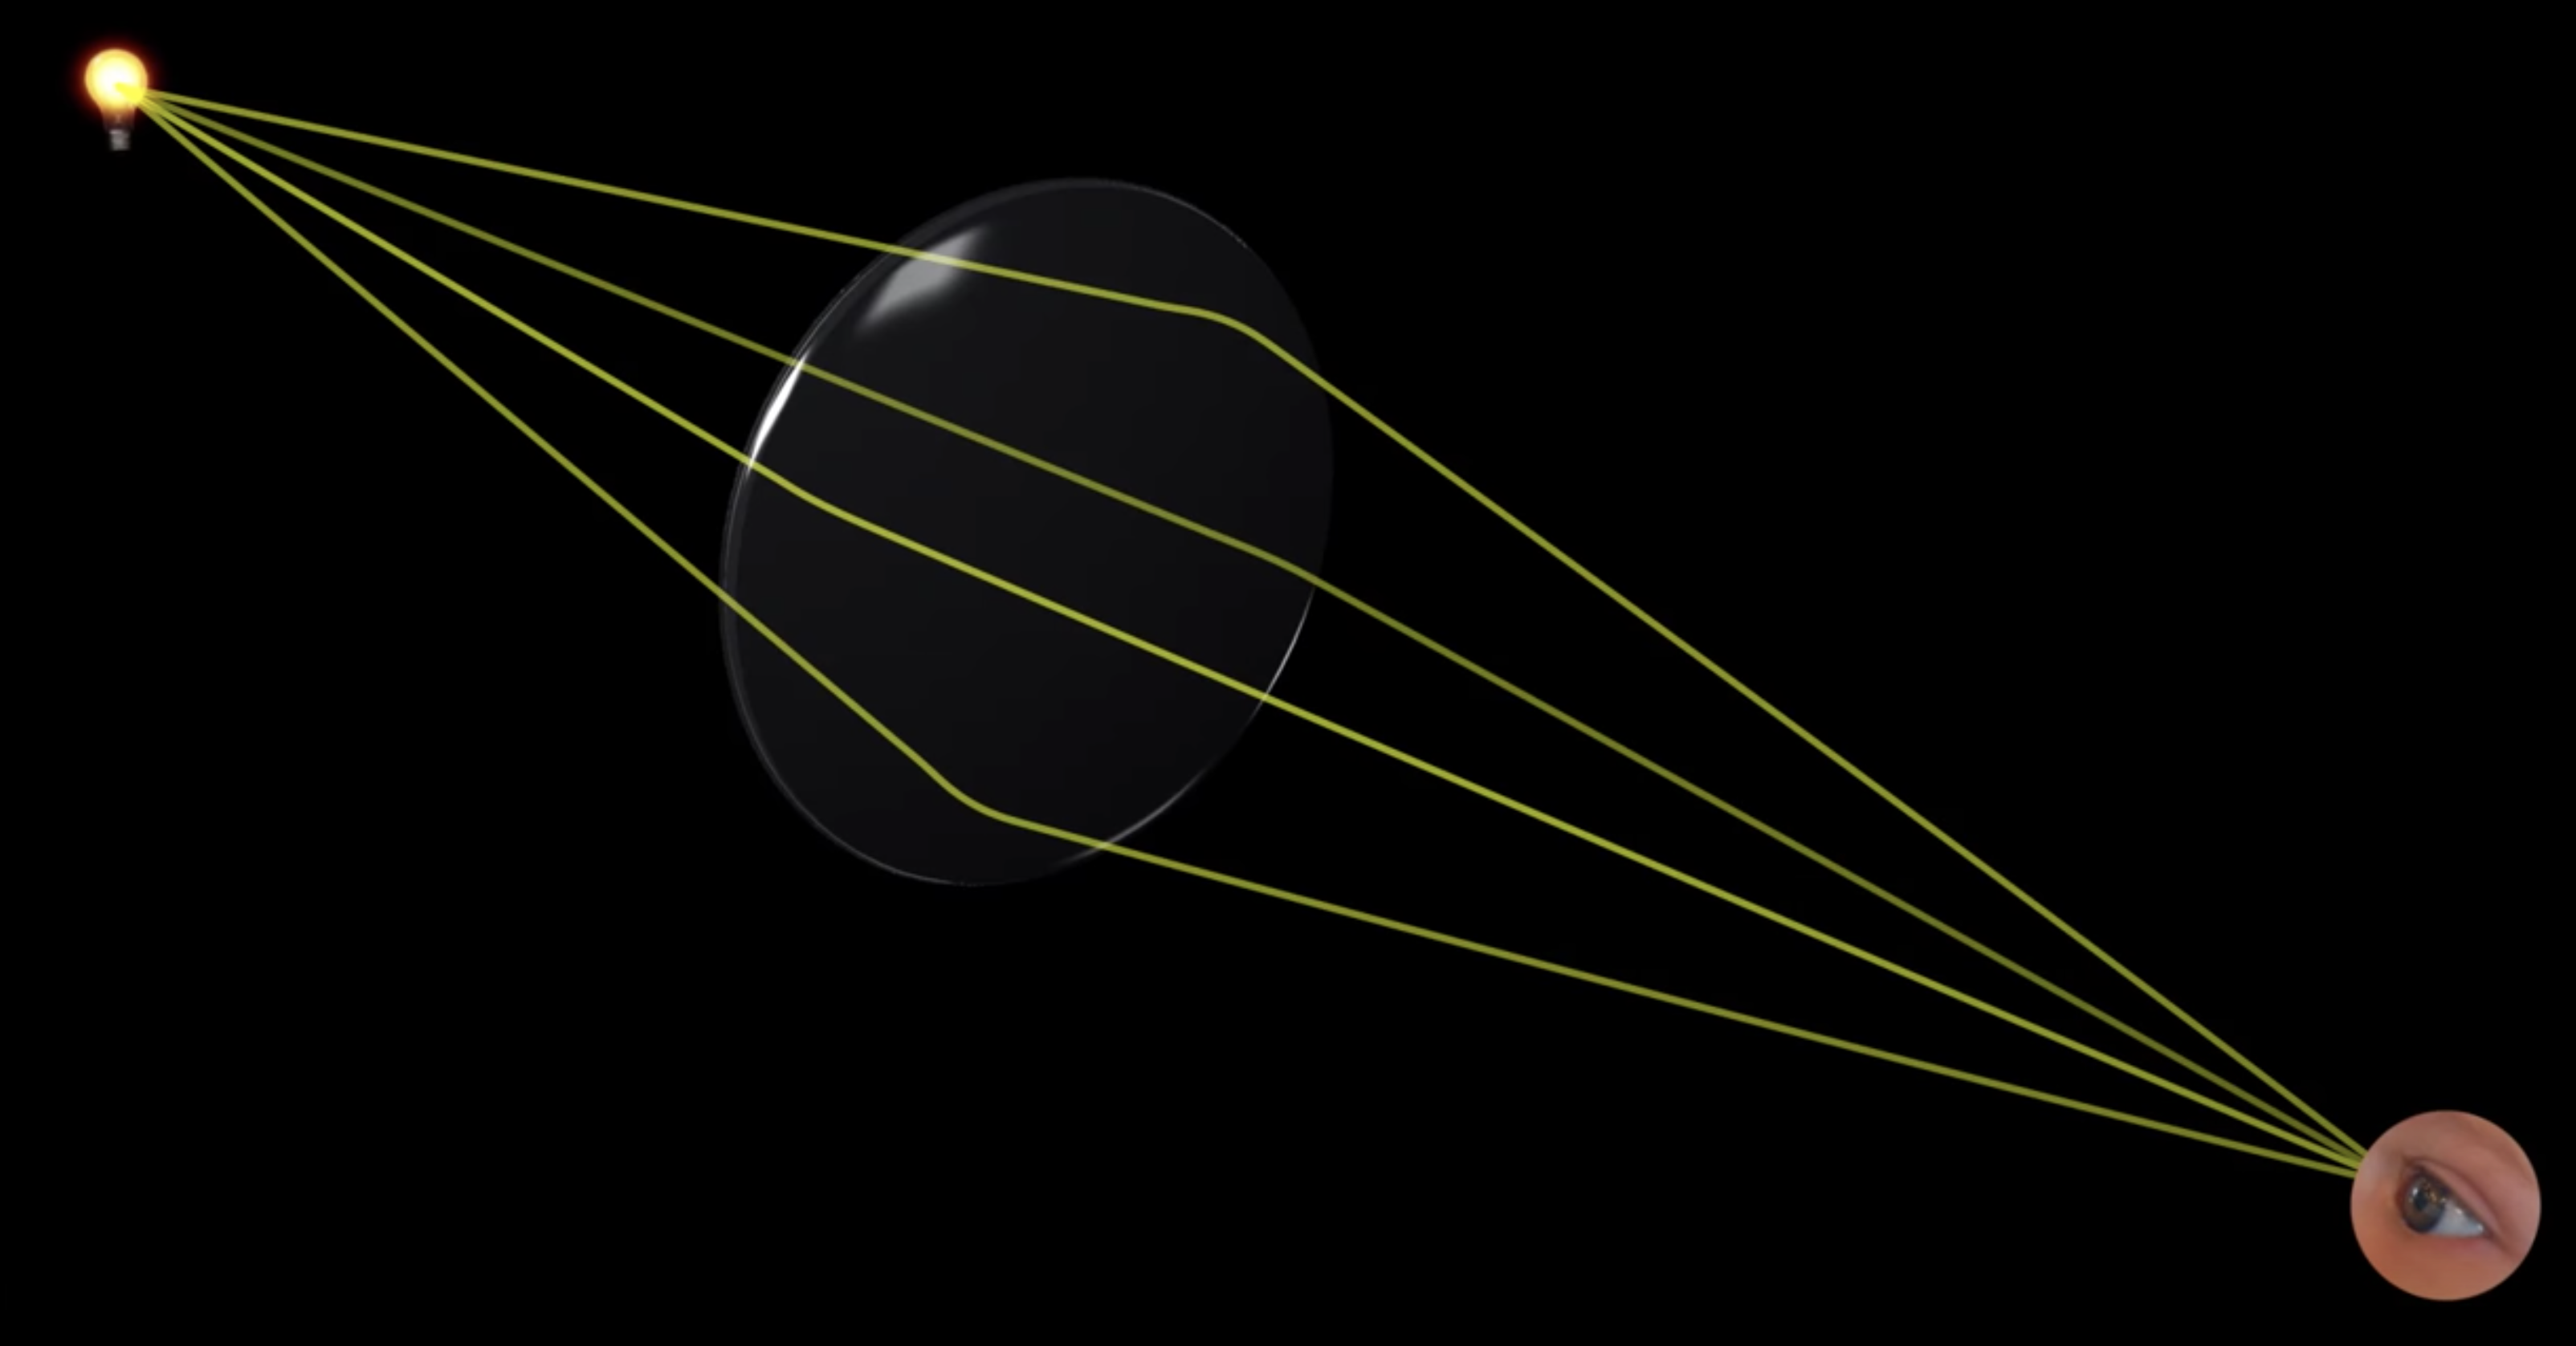
\includegraphics[width=0.49  \textwidth]{lens1}
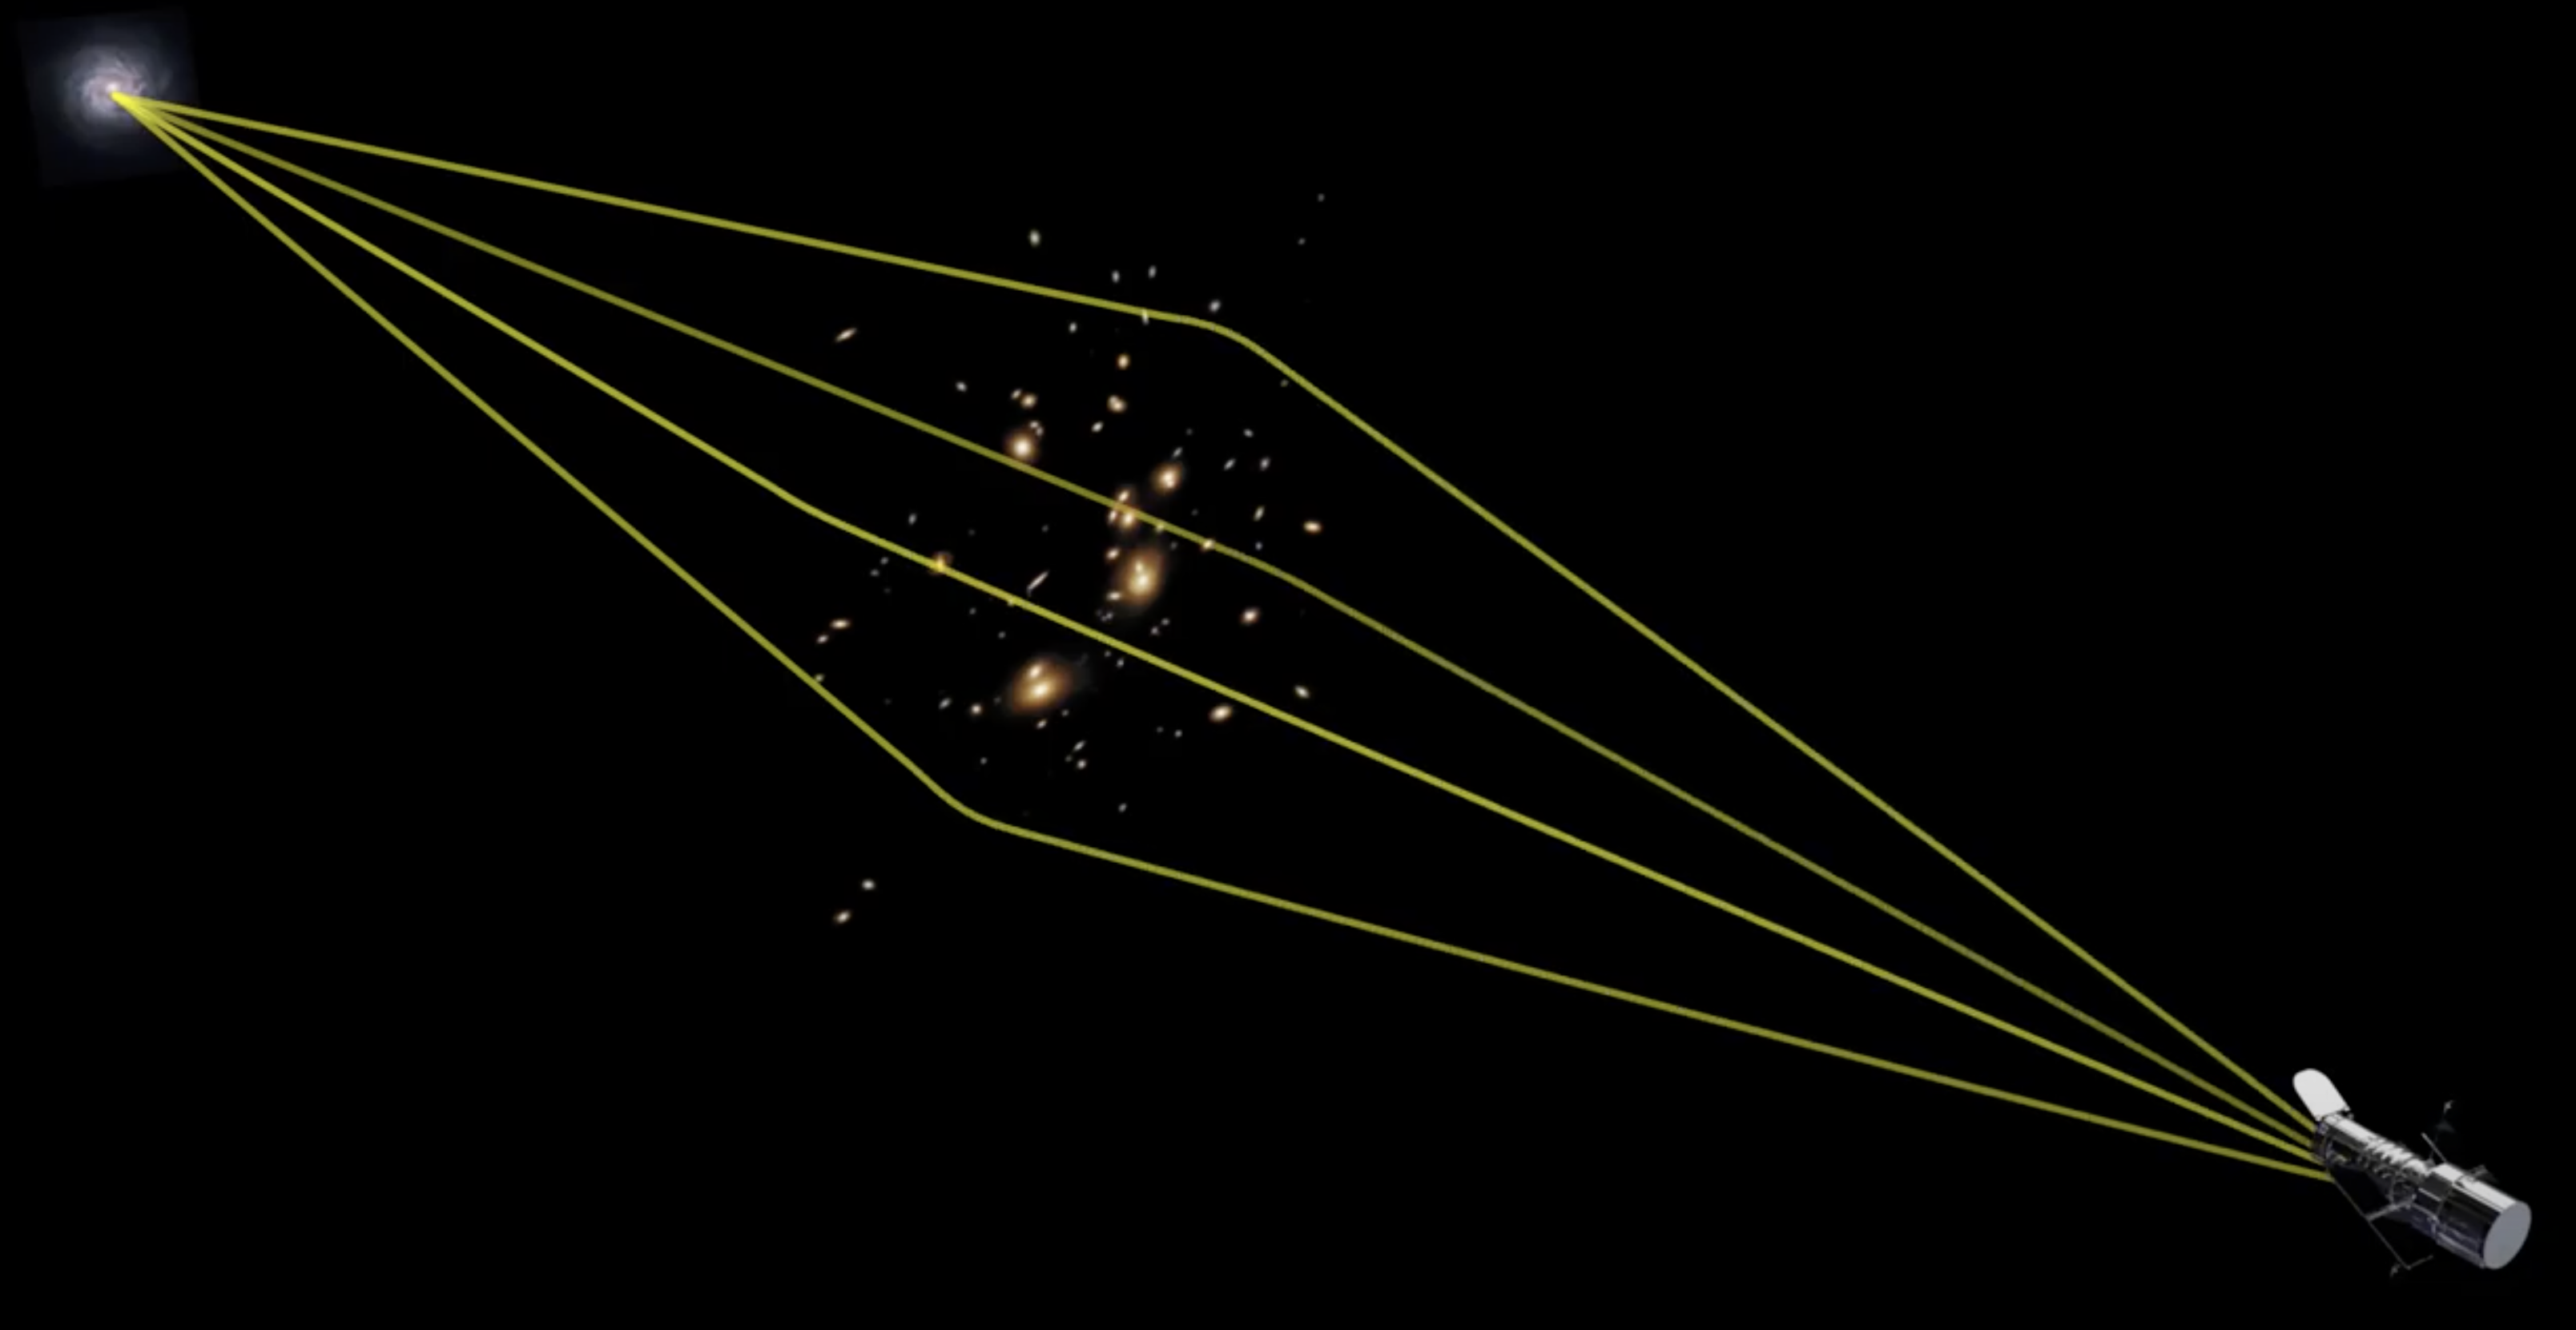
\includegraphics[width=0.49\textwidth]{lens2}
\caption{Ilustración do `efecto lente'. Na esquerda vemos como funciona una lente de verdade, como 
as que usamos no día a día, cambiando o camiño que segue a luz de camiño aos nosos ollos, e de esta forma 
distorsionando a imaxe. Na dereita vemos como a materia escura fai o mesmo cas imaxes de galaxias, 
distorsionándoas no seu camiño ao telescopio. Imaxe: {\it Hubble Space Telescope}, \url{https://hubblesite.org/}
\label{fig:lens_example}
}
\end{figure}

Polo tanto, a pesar de que non podemos ver a materia escura directamente, podemos vela indirectamente, 
a través de este `efecto lente' (en inglés {\it lensing}, derivado da palabra {\it lens}, que significa 
lente), ilustrado na figura \ref{fig:lens_example}. Porén, ai outro problema. Se as galaxias foran 
perfectas esferas, como un balón de fútbol, sería moi fácil saber como de distorsionadas están. Pero en 
realidade, a maioría das galaxias son elípticas, como un ovo. Polo tanto, cando usamos un telescopio e 
vemos una galaxia que parece `estirada', é imposible saber se esta estirada porque estamos mirando a través 
dunha lente de materia escura, ou se está estirada porque esa é a súa forma real. A solución a este problema 
e mirar non solo unha, senón millóns de galaxias. Se varias galaxias próximas están alongadas na mesma 
dirección, é moi pouco probable que por casualidade, todas teñan a mesma forma, e apunten na o mesmo sitio.
Nese caso, sabemos que estamos observando esas galaxias a través dunha lente. E polo tanto, indirectamente, 
estamos vendo a invisible materia escura.

Na última década foi posible observar o ceo como nunca antes, grazas a grandes avances tecnolóxicos e 
científicos, e importantes inversións por parte dos gobernos de varios países. Un exemplo disto é a {\it Dark 
Energy Survey}, abreviado como DES, una colaboración de varias institucións académicas en múltiples países, incluídas
varias españolas, que utilizou o Telescopio Víctor Manuel Blanco en Chile para observar aproximadamente 300 millóns de galaxias, utilizando 
unha técnica chamada fotometría. Utilizando esta gran cantidade de imaxes, e avanzados métodos estadísticos, DES 
logrou, entre outras cosas, crear un mapa da materia escura vista dende a nosa galaxia. O mapa, mostrado na figura
 \ref{fig:massmap}, mostra a cantidade de materia escura, vista dende distintos puntos no ceo. As zonas azuis son áreas 
 con menos materia escura, e as zonas vermellas teñen máis. Seguro que se estas vendo esta imaxe recórdate a algo, 
 como cando ves as nubes e buscas formas. Moita xente pensa nunha arañeira, por iso coloquialmente chamámoslle a 
 arañeira cósmica ({\it cosmic web} en inglés). 

Nos próximos anos, telescopios aínda máis potentes que DES mellorarán estas primeiras imaxes da materia escura, 
observando moitas máis galaxias con superior precisión. O noso obxectivo segue sendo descubrir de que está feito 
este misterioso e invisible compoñente do Universo, que é moito máis común que a materia que coñecemos. Quizais 
algún día, dende o noso pequeno planeta, podamos descifrar de que está feito o Universo. De momento, por primeira 
vez, podemos ver o invisible. 

\begin{figure}[h]
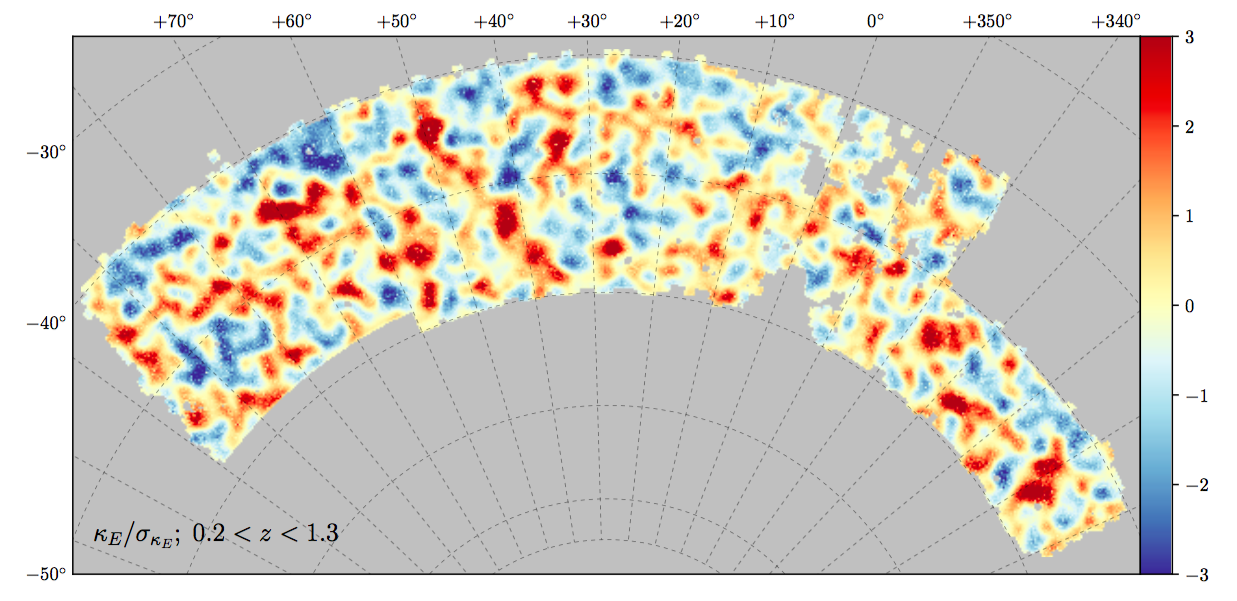
\includegraphics[width=\textwidth]{Y1-massmap}
\caption{Mapa da materia escura observado por DES. Imaxe: \cite{chang}.
\label{fig:massmap}
}
\end{figure}

\bibliographystyle{apalike}
\bibliography{ag}

\end{document}
